\begin{activity} \label{A:9.1.7}

 \begin{figure}[ht]
\begin{center}
\resizebox{!}{2.0in}{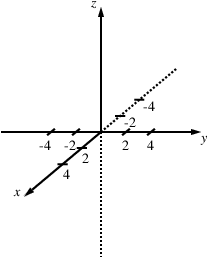
\includegraphics{figures/9_1_traces_activity_1}}
\caption{Coordinate axes to sketch traces.}
\label{F:9.1.traces_activity_1}
\end{center}
\end{figure}
   \ba
   \item Identify the traces in the $x$ direction (keeping $y$ constant). Draw the $y=-4$, $y=-2$, $y=0$, $y=2$, and $y=4$ traces in 3-dimensional coordinate system in Figure \ref{F:9.1.traces_activity_1}.

    \item Identify the traces in the $y$ direction (keeping $x$ constant). Draw the $x=-4$, $x=-2$, $x=0$, $x=2$, and $x=4$ traces in 3-dimensional coordinate system in Figure \ref{F:9.1.traces_activity_1}.

    \item Describe the surface defined by the function $f$.

     \ea

\end{activity}
\begin{smallhint}

\end{smallhint}
\begin{bighint}

\end{bighint}
\begin{activitySolution}


\end{activitySolution}
\aftera 